% From https://github.com/LSSTDESC/name-tag-guru

% Ti use transparent with xelatex
\RequirePackage{pdfmanagement-testphase}
\DeclareDocumentMetadata{}

\documentclass[letterpaper,10pt]{article}

%% To include CJK character, one needs to use xelatex to compile
%% and also to have a CJK font installed (current set to `Noto Sans CJK TC`)
%% Otherwise, comment out the following two lines.
%\usepackage{xeCJK}
%\setCJKmainfont{Noto Sans CJK TC}

%% basic font settings
\usepackage[T1]{fontenc}
\usepackage[default]{raleway}
\providecommand{\raleway}{} % in case we are not using xeLaTex
\newcommand*{\latinfont}{\raleway}
\hyphenpenalty=10000

%% essential packages
\usepackage[boxed]{ticket} %Remove the [boxed] option to remove the badge boundary for printing
\usepackage[usenames,dvipsnames]{xcolor}
\usepackage{graphicx} % provides \includegraphics
\usepackage{adjustbox} % provides \maxsizebox

%% To make background partially transparent
\usepackage{transparent}

%% to use colored text for highlighting
\newcommand*{\highlight}{\textcolor}
%% OR, to use contour for highlighting, uncomment below
%\usepackage[outline]{contour}
%\contourlength{5pt}
%\newcommand*{\highlight}{\contour}

%% other useful commands
\newcommand*{\cbox}[1]{\makebox[0pt]{\maxsizebox{3.8in}{!}{#1}}}
\newcommand*{\lbox}[1]{\makebox[0pt][l]{\maxsizebox{3.8in}{!}{#1}}}
\newcommand*{\rbox}[1]{\makebox[0pt][r]{\maxsizebox{3.8in}{!}{#1}}}
\newcommand*{\largefont}{\fontsize{68pt}{0pt}\selectfont}
\newcommand*{\smallfont}{\fontsize{26pt}{0pt}\selectfont}
\newcommand*{\infofont}{\fontsize{22pt}{0pt}\selectfont}

%% page setting, currently set to match Avery Name Badges #74459
\hoffset=-0.75in %adjusting page margin
\voffset=-0.125in %adjusting page margin
\unitlength=0.01in
\ticketSize{400}{300} % in unitlength
\ticketDistance{0}{0} %in unitlength
\ticketNumbers{2}{3} % how many badges per page

%% ticket default setting
\renewcommand*{\ticketdefault}{%
  \put(10,2){\lbox{{\transparent{0.2}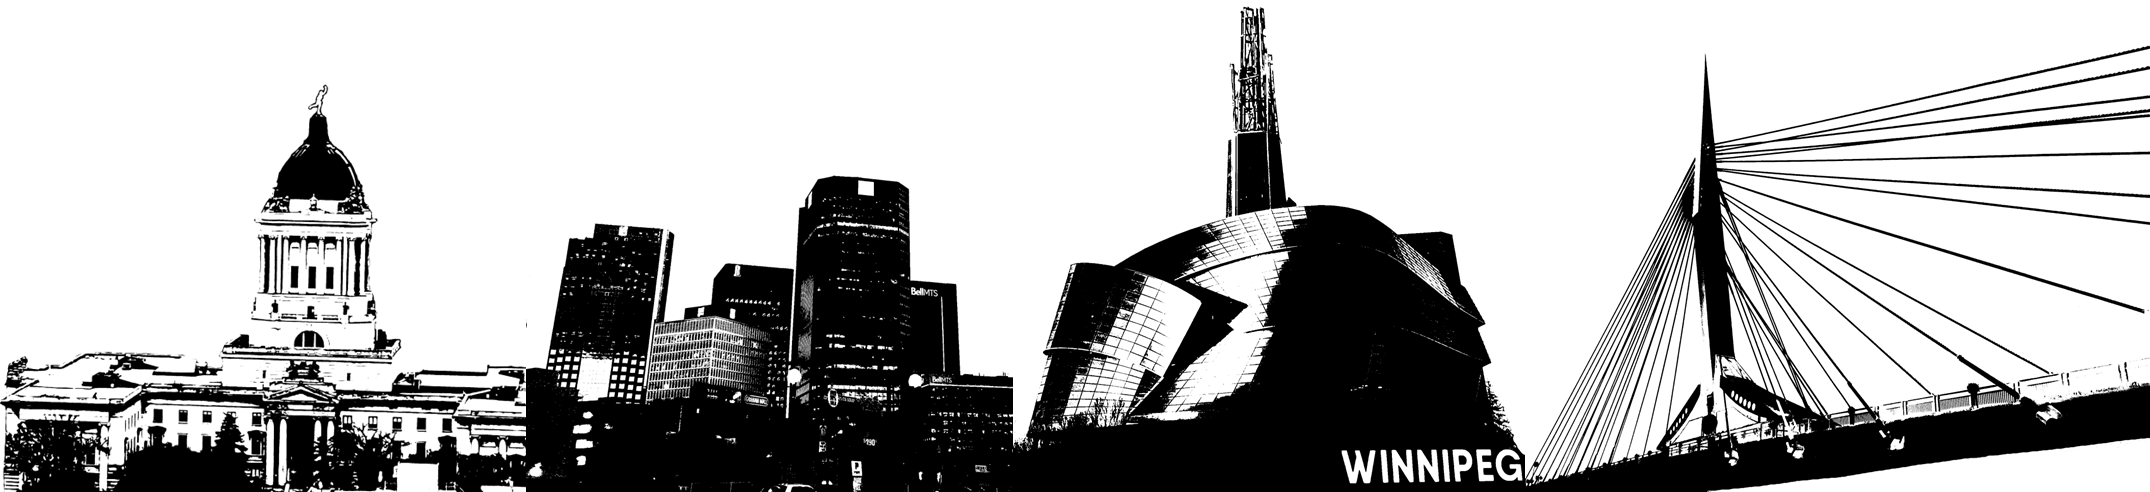
\includegraphics[width=\textwidth]{SkylineWinnipgeLong}}}}%
  \put(205,29){\cbox{\latinfont\small Computational and Mathematical Population Dynamics 6}}% Update dates as needed
  \put(205,15){\cbox{\latinfont\footnotesize University of Manitoba, 23--27 May 2023}}% Update location as needed
}

%% participant style setting
\newcommand*{\participant}[5]{\ticket{%
  \put(200,210){\cbox{#5{\latinfont\bfseries\largefont #1}}}%
  \put(200,155){\cbox{#5{\latinfont\bfseries\smallfont #2}}}%
  \put(200,106){\cbox{\latinfont\infofont #3}}%
  \put(200,62){\cbox{\latinfont\infofont #4}}%
}}

%% empty ticket (with background)
\newcommand*{\emptyticket}{\ticket{}}

%% local people or other highlight commands
\newcommand*{\local}{\highlight{orange}}
\newcommand*{\contact}{\highlight{CornflowerBlue}}


%% backside printing (comment out for front side)
\hoffset=1.1in
\backside

\begin{document}
%%%%%%%%%%%%%%%%%%%%%%%%%%%%%%%%%%%
% insert below the participant list
%%%%%%%%%%%%%%%%%%%%%%%%%%%%%%%%%%%
\participant{Azmy}{Ackleh}{University of Louisiana - Lafayette}{(\qquad | \qquad)}{}
\participant{Folashade}{Agusto}{University of Kansas}{(\qquad | \qquad)}{}
\participant{Ephraim}{Agyingi}{Rochester Institute of Technology}{(\qquad | \qquad)}{}
\participant{Azmy}{Ackleh}{University of Louisiana - Lafayette}{(\qquad | \qquad)}{}
\participant{Folashade}{Agusto}{University of Kansas}{(\qquad | \qquad)}{}
\participant{Ephraim}{Agyingi}{Rochester Institute of Technology}{(\qquad | \qquad)}{}
\participant{Vitalii}{Akimenko}{University of Manitoba}{(\qquad | \qquad)}{}
\participant{Asami}{Anzai}{Kyoto University}{(\qquad | \qquad)}{}
\participant{Julien}{Arino}{University of Manitoba}{(\qquad | \qquad)}{}
\participant{Vitalii}{Akimenko}{University of Manitoba}{(\qquad | \qquad)}{}
\participant{Asami}{Anzai}{Kyoto University}{(\qquad | \qquad)}{}
\participant{Julien}{Arino}{University of Manitoba}{(\qquad | \qquad)}{}
\participant{Joseph}{Baafi}{Memorial University}{(\qquad | \qquad)}{}
\participant{Jacques}{Bélair}{Université de Montréal}{(\qquad | \qquad)}{}
\participant{Ranjini}{Bhattacharya}{Moffitt Cancer Center}{(\qquad | \qquad)}{}
\participant{Joseph}{Baafi}{Memorial University}{(\qquad | \qquad)}{}
\participant{Jacques}{Bélair}{Université de Montréal}{(\qquad | \qquad)}{}
\participant{Ranjini}{Bhattacharya}{Moffitt Cancer Center}{(\qquad | \qquad)}{}
\participant{Tijotop Ahmed}{Binjibon}{University of Manitoba}{(\qquad | \qquad)}{}
\participant{Amanda}{Bleichrodt}{Georgia State University}{(\qquad | \qquad)}{}
\participant{Ernesto Augusto}{Bueno da Fonseca Lima}{The University of Texas at Austin}{(\qquad | \qquad)}{}
\participant{Tijotop Ahmed}{Binjibon}{University of Manitoba}{(\qquad | \qquad)}{}
\participant{Amanda}{Bleichrodt}{Georgia State University}{(\qquad | \qquad)}{}
\participant{Ernesto Augusto}{Bueno da Fonseca Lima}{The University of Texas at Austin}{(\qquad | \qquad)}{}
\participant{Anuraag}{Bukkuri}{Moffitt Cancer Center}{(\qquad | \qquad)}{}
\participant{Robert Stephen}{Cantrell}{University of Miami}{(\qquad | \qquad)}{}
\participant{Erwing}{Cardozo-Ojeda}{Fred Hutchinson Cancer Center}{(\qquad | \qquad)}{}
\participant{Anuraag}{Bukkuri}{Moffitt Cancer Center}{(\qquad | \qquad)}{}
\participant{Robert Stephen}{Cantrell}{University of Miami}{(\qquad | \qquad)}{}
\participant{Erwing}{Cardozo-Ojeda}{Fred Hutchinson Cancer Center}{(\qquad | \qquad)}{}
\participant{Bernard}{Cazelles}{IRD Sorbonne Université}{(\qquad | \qquad)}{}
\participant{Stanca}{Ciupe}{Virginia Tech}{(\qquad | \qquad)}{}
\participant{Adriana-Stefania}{Ciupeanu}{University of Manitoba}{(\qquad | \qquad)}{}
\participant{Bernard}{Cazelles}{IRD Sorbonne Université}{(\qquad | \qquad)}{}
\participant{Stanca}{Ciupe}{Virginia Tech}{(\qquad | \qquad)}{}
\participant{Adriana-Stefania}{Ciupeanu}{University of Manitoba}{(\qquad | \qquad)}{}
\participant{Jessica}{Conway}{Penn State}{(\qquad | \qquad)}{}
\participant{Morgan}{Craig}{Sainte-Justine University Hopsital Research Centre / Université de Montréal}{(\qquad | \qquad)}{}
\participant{Jim}{Cushing}{University of Arizona}{(\qquad | \qquad)}{}
\participant{Jessica}{Conway}{Penn State}{(\qquad | \qquad)}{}
\participant{Morgan}{Craig}{Sainte-Justine University Hopsital Research Centre / Université de Montréal}{(\qquad | \qquad)}{}
\participant{Jim}{Cushing}{University of Arizona}{(\qquad | \qquad)}{}
\participant{Tanuja}{Das}{University of New Brunswick}{(\qquad | \qquad)}{}
\participant{Xiaoyan}{Deng}{Université de Montréal}{(\qquad | \qquad)}{}
\participant{Clotilde}{Djuikem}{INRIA BIOCORE}{(\qquad | \qquad)}{}
\participant{Tanuja}{Das}{University of New Brunswick}{(\qquad | \qquad)}{}
\participant{Xiaoyan}{Deng}{Université de Montréal}{(\qquad | \qquad)}{}
\participant{Clotilde}{Djuikem}{INRIA BIOCORE}{(\qquad | \qquad)}{}
\participant{Marisa}{Eisenberg}{University of Michigan, Ann Arbor}{(\qquad | \qquad)}{}
\participant{Guihong}{Fan}{Columbus State Unvierstiy}{(\qquad | \qquad)}{}
\participant{Suzan}{Farhang-Sardroodi}{university of Manitoba}{(\qquad | \qquad)}{}
\participant{Marisa}{Eisenberg}{University of Michigan, Ann Arbor}{(\qquad | \qquad)}{}
\participant{Guihong}{Fan}{Columbus State Unvierstiy}{(\qquad | \qquad)}{}
\participant{Suzan}{Farhang-Sardroodi}{university of Manitoba}{(\qquad | \qquad)}{}
\participant{Ghazale}{Farjam}{University of Manitoba}{(\qquad | \qquad)}{}
\participant{Jonathan}{Forde}{Hobart and William Smith Colleges}{(\qquad | \qquad)}{}
\participant{Samaneh}{Gholami}{York University}{(\qquad | \qquad)}{}
\participant{Ghazale}{Farjam}{University of Manitoba}{(\qquad | \qquad)}{}
\participant{Jonathan}{Forde}{Hobart and William Smith Colleges}{(\qquad | \qquad)}{}
\participant{Samaneh}{Gholami}{York University}{(\qquad | \qquad)}{}
\participant{Abba}{Gumel}{UMD}{(\qquad | \qquad)}{}
\participant{Donglin}{Han}{University of Alberta}{(\qquad | \qquad)}{}
\participant{Md. Mehadi}{Hasan}{University of Manitoba}{(\qquad | \qquad)}{}
\participant{Abba}{Gumel}{UMD}{(\qquad | \qquad)}{}
\participant{Donglin}{Han}{University of Alberta}{(\qquad | \qquad)}{}
\participant{Md. Mehadi}{Hasan}{University of Manitoba}{(\qquad | \qquad)}{}
\participant{Katsuma}{Hayashi}{Kyoto-U}{(\qquad | \qquad)}{}
\participant{Jane}{Heffernan}{York University}{(\qquad | \qquad)}{}
\participant{Esteban A.}{Hernandez-Vargas}{University of Idaho}{(\qquad | \qquad)}{}
\participant{Katsuma}{Hayashi}{Kyoto-U}{(\qquad | \qquad)}{}
\participant{Jane}{Heffernan}{York University}{(\qquad | \qquad)}{}
\participant{Esteban A.}{Hernandez-Vargas}{University of Idaho}{(\qquad | \qquad)}{}
\participant{Thomas}{Hillen}{University of Alberta}{(\qquad | \qquad)}{}
\participant{Jannatun Irana}{Ira}{University of Manitoba}{(\qquad | \qquad)}{}
\participant{Sarafa}{Iyaniwura}{University of British Columbia, Vancouver}{(\qquad | \qquad)}{}
\participant{Thomas}{Hillen}{University of Alberta}{(\qquad | \qquad)}{}
\participant{Jannatun Irana}{Ira}{University of Manitoba}{(\qquad | \qquad)}{}
\participant{Sarafa}{Iyaniwura}{University of British Columbia, Vancouver}{(\qquad | \qquad)}{}
\participant{Harsh}{Jain}{University of Minnesota Duluth}{(\qquad | \qquad)}{}
\participant{Ali}{Karoobi}{University of Manitoba}{(\qquad | \qquad)}{}
\participant{Marek}{Kimmel}{Rice University}{(\qquad | \qquad)}{}
\participant{Harsh}{Jain}{University of Minnesota Duluth}{(\qquad | \qquad)}{}
\participant{Ali}{Karoobi}{University of Manitoba}{(\qquad | \qquad)}{}
\participant{Marek}{Kimmel}{Rice University}{(\qquad | \qquad)}{}
\participant{Jude}{Kong}{York University}{(\qquad | \qquad)}{}
\participant{Chapin}{Korosec}{Simon Fraser University}{(\qquad | \qquad)}{}
\participant{Christopher}{Kribs}{University of Texas at Arlington}{(\qquad | \qquad)}{}
\participant{Jude}{Kong}{York University}{(\qquad | \qquad)}{}
\participant{Chapin}{Korosec}{Simon Fraser University}{(\qquad | \qquad)}{}
\participant{Christopher}{Kribs}{University of Texas at Arlington}{(\qquad | \qquad)}{}
\participant{Brandon}{Legried}{Georgia Institute of Technology}{(\qquad | \qquad)}{}
\participant{Kang-Ling}{Liao}{University of Manitoba}{(\qquad | \qquad)}{}
\participant{Xiaochen}{Long}{Rice University}{(\qquad | \qquad)}{}
\participant{Brandon}{Legried}{Georgia Institute of Technology}{(\qquad | \qquad)}{}
\participant{Kang-Ling}{Liao}{University of Manitoba}{(\qquad | \qquad)}{}
\participant{Xiaochen}{Long}{Rice University}{(\qquad | \qquad)}{}
\participant{Pedro}{Lopez Gascon}{University of Manitoba}{(\qquad | \qquad)}{}
\participant{Loïc}{Louison}{Université de Guyane}{(\qquad | \qquad)}{}
\participant{Nadia}{Loy}{Politecnico di Torino}{(\qquad | \qquad)}{}
\participant{Pedro}{Lopez Gascon}{University of Manitoba}{(\qquad | \qquad)}{}
\participant{Loïc}{Louison}{Université de Guyane}{(\qquad | \qquad)}{}
\participant{Nadia}{Loy}{Politecnico di Torino}{(\qquad | \qquad)}{}
\participant{Chinwendu Emilian}{Madubueze}{York University  Toronto}{(\qquad | \qquad)}{}
\participant{Solomon}{mensah}{University of Manitoba}{(\qquad | \qquad)}{}
\participant{Fabio}{Milner}{Arizona State University}{(\qquad | \qquad)}{}
\participant{Chinwendu Emilian}{Madubueze}{York University  Toronto}{(\qquad | \qquad)}{}
\participant{Solomon}{mensah}{University of Manitoba}{(\qquad | \qquad)}{}
\participant{Fabio}{Milner}{Arizona State University}{(\qquad | \qquad)}{}
\participant{Negar}{Mohammadnejad}{university of manitoba}{(\qquad | \qquad)}{}
\participant{Jemal}{Mohammed-Awel}{Morgan State University}{(\qquad | \qquad)}{}
\participant{Nicola}{Mulberry}{Simon Fraser}{(\qquad | \qquad)}{}
\participant{Negar}{Mohammadnejad}{university of manitoba}{(\qquad | \qquad)}{}
\participant{Jemal}{Mohammed-Awel}{Morgan State University}{(\qquad | \qquad)}{}
\participant{Nicola}{Mulberry}{Simon Fraser}{(\qquad | \qquad)}{}
\participant{Toshiyuki}{Namba}{Osaka Metropolitan University}{(\qquad | \qquad)}{}
\participant{Syeda Atika Batool}{Naqvi}{University of Manitoba}{(\qquad | \qquad)}{}
\participant{Jay}{Newby}{University of Alberta}{(\qquad | \qquad)}{}
\participant{Toshiyuki}{Namba}{Osaka Metropolitan University}{(\qquad | \qquad)}{}
\participant{Syeda Atika Batool}{Naqvi}{University of Manitoba}{(\qquad | \qquad)}{}
\participant{Jay}{Newby}{University of Alberta}{(\qquad | \qquad)}{}
\participant{Hiroshi}{Nishiura}{Kyoto University}{(\qquad | \qquad)}{}
\participant{Ryo}{Oizumi}{National Institute of Population and Social Security Research}{(\qquad | \qquad)}{}
\participant{Lorenzo}{Pellis}{The University of Manchester}{(\qquad | \qquad)}{}
\participant{Hiroshi}{Nishiura}{Kyoto University}{(\qquad | \qquad)}{}
\participant{Ryo}{Oizumi}{National Institute of Population and Social Security Research}{(\qquad | \qquad)}{}
\participant{Lorenzo}{Pellis}{The University of Manchester}{(\qquad | \qquad)}{}
\participant{Tin}{Phan}{Los Alamos National Laboratory}{(\qquad | \qquad)}{}
\participant{Tanya}{Philippsen}{University of Victoria}{(\qquad | \qquad)}{}
\participant{Stephanie}{Portet}{University of Manitoba}{(\qquad | \qquad)}{}
\participant{Tin}{Phan}{Los Alamos National Laboratory}{(\qquad | \qquad)}{}
\participant{Tanya}{Philippsen}{University of Victoria}{(\qquad | \qquad)}{}
\participant{Stephanie}{Portet}{University of Manitoba}{(\qquad | \qquad)}{}
\participant{Andrea}{Pugliese}{Università degli Studi di Trento}{(\qquad | \qquad)}{}
\participant{Erica}{Rutter}{University of California, Merced}{(\qquad | \qquad)}{}
\participant{Paul}{Salceanu}{University of Louisiana at Lafayette}{(\qquad | \qquad)}{}
\participant{Andrea}{Pugliese}{Università degli Studi di Trento}{(\qquad | \qquad)}{}
\participant{Erica}{Rutter}{University of California, Merced}{(\qquad | \qquad)}{}
\participant{Paul}{Salceanu}{University of Louisiana at Lafayette}{(\qquad | \qquad)}{}
\participant{Leili}{Shahriyari}{University of Massachusetts Amherst}{(\qquad | \qquad)}{}
\participant{Zhisheng}{Shuai}{University of Central Florida}{(\qquad | \qquad)}{}
\participant{Nourridine}{Siewe}{Rochester Institute of Technology}{(\qquad | \qquad)}{}
\participant{Leili}{Shahriyari}{University of Massachusetts Amherst}{(\qquad | \qquad)}{}
\participant{Zhisheng}{Shuai}{University of Central Florida}{(\qquad | \qquad)}{}
\participant{Nourridine}{Siewe}{Rochester Institute of Technology}{(\qquad | \qquad)}{}
\participant{Stacey}{Smith}{The University of Ottawa}{(\qquad | \qquad)}{}
\participant{Tracy}{Stepien}{University of Florida}{(\qquad | \qquad)}{}
\participant{Yasuhiro}{Takeushi}{Aoyama Gakuin University}{(\qquad | \qquad)}{}
\participant{Stacey}{Smith}{The University of Ottawa}{(\qquad | \qquad)}{}
\participant{Tracy}{Stepien}{University of Florida}{(\qquad | \qquad)}{}
\participant{Yasuhiro}{Takeushi}{Aoyama Gakuin University}{(\qquad | \qquad)}{}
\participant{Ryan}{Thiessen}{University of Alberta}{(\qquad | \qquad)}{}
\participant{Sonja}{Tuerpitz}{Friedrich Schiller University Jena}{(\qquad | \qquad)}{}
\participant{Necibe}{Tuncer}{FAU}{(\qquad | \qquad)}{}
\participant{Ryan}{Thiessen}{University of Alberta}{(\qquad | \qquad)}{}
\participant{Sonja}{Tuerpitz}{Friedrich Schiller University Jena}{(\qquad | \qquad)}{}
\participant{Necibe}{Tuncer}{FAU}{(\qquad | \qquad)}{}
\participant{Pauline}{van den Driessche}{University of Victoria}{(\qquad | \qquad)}{}
\participant{Marie Betsy}{Varughese}{University of Alberta}{(\qquad | \qquad)}{}
\participant{Jorge}{Velasco-Hernandez}{UNAM}{(\qquad | \qquad)}{}
\participant{Pauline}{van den Driessche}{University of Victoria}{(\qquad | \qquad)}{}
\participant{Marie Betsy}{Varughese}{University of Alberta}{(\qquad | \qquad)}{}
\participant{Jorge}{Velasco-Hernandez}{UNAM}{(\qquad | \qquad)}{}
\participant{Amy}{Veprauskas}{University of LA at Lafayette}{(\qquad | \qquad)}{}
\participant{Ren-Yi}{Wang}{Rice University}{(\qquad | \qquad)}{}
\participant{Xuyuan}{Wang}{University of Alberta}{(\qquad | \qquad)}{}
\participant{Amy}{Veprauskas}{University of LA at Lafayette}{(\qquad | \qquad)}{}
\participant{Ren-Yi}{Wang}{Rice University}{(\qquad | \qquad)}{}
\participant{Xuyuan}{Wang}{University of Alberta}{(\qquad | \qquad)}{}
\participant{Kenton}{Watt}{University of Manitoba}{(\qquad | \qquad)}{}
\participant{Adam}{Wieler}{University of Manitoba}{(\qquad | \qquad)}{}
\participant{Kathleen}{Wilkie}{Toronto Metropolitan University}{(\qquad | \qquad)}{}
\participant{Kenton}{Watt}{University of Manitoba}{(\qquad | \qquad)}{}
\participant{Adam}{Wieler}{University of Manitoba}{(\qquad | \qquad)}{}
\participant{Kathleen}{Wilkie}{Toronto Metropolitan University}{(\qquad | \qquad)}{}
\participant{Xiangye}{Xu}{University of Manitoba}{(\qquad | \qquad)}{}
\participant{Pei}{Yuan}{York University}{(\qquad | \qquad)}{}
\participant{Veronika}{Zarnitsyna}{Emory University}{(\qquad | \qquad)}{}
\participant{Xiangye}{Xu}{University of Manitoba}{(\qquad | \qquad)}{}
\participant{Pei}{Yuan}{York University}{(\qquad | \qquad)}{}
\participant{Veronika}{Zarnitsyna}{Emory University}{(\qquad | \qquad)}{}
\participant{NA}{NA}{NA}{(\qquad | \qquad)}{}
\participant{NA}{NA}{NA}{(\qquad | \qquad)}{}

%%%%%%%%%%%%%%%%%%%%%%%%%%%%%%%%%%%
% end of the participant list
%%%%%%%%%%%%%%%%%%%%%%%%%%%%%%%%%%%
% empty tickets below
%\emptyticket{}
%\emptyticket{}
\end{document}
